\documentclass[../../labo_tp5_main.tex]{subfiles}

\begin{document}

%capítulo
\section{Ejercicio 4}

Se procedi\'o a observar el espectro de se\~nales moduladas en FM. Al igual que el caso anterior, se utiliz\'o una portadora senoidal de frecuencia 1.9MHz con amplitud 200m$\mathrm{V}_{\mathrm{pp}}$

En primer lugar, se utiliz\'o como moduladora una se\~nal senoidal de 100kHz.

\begin{figure}[H]
	\centering
	\fbox{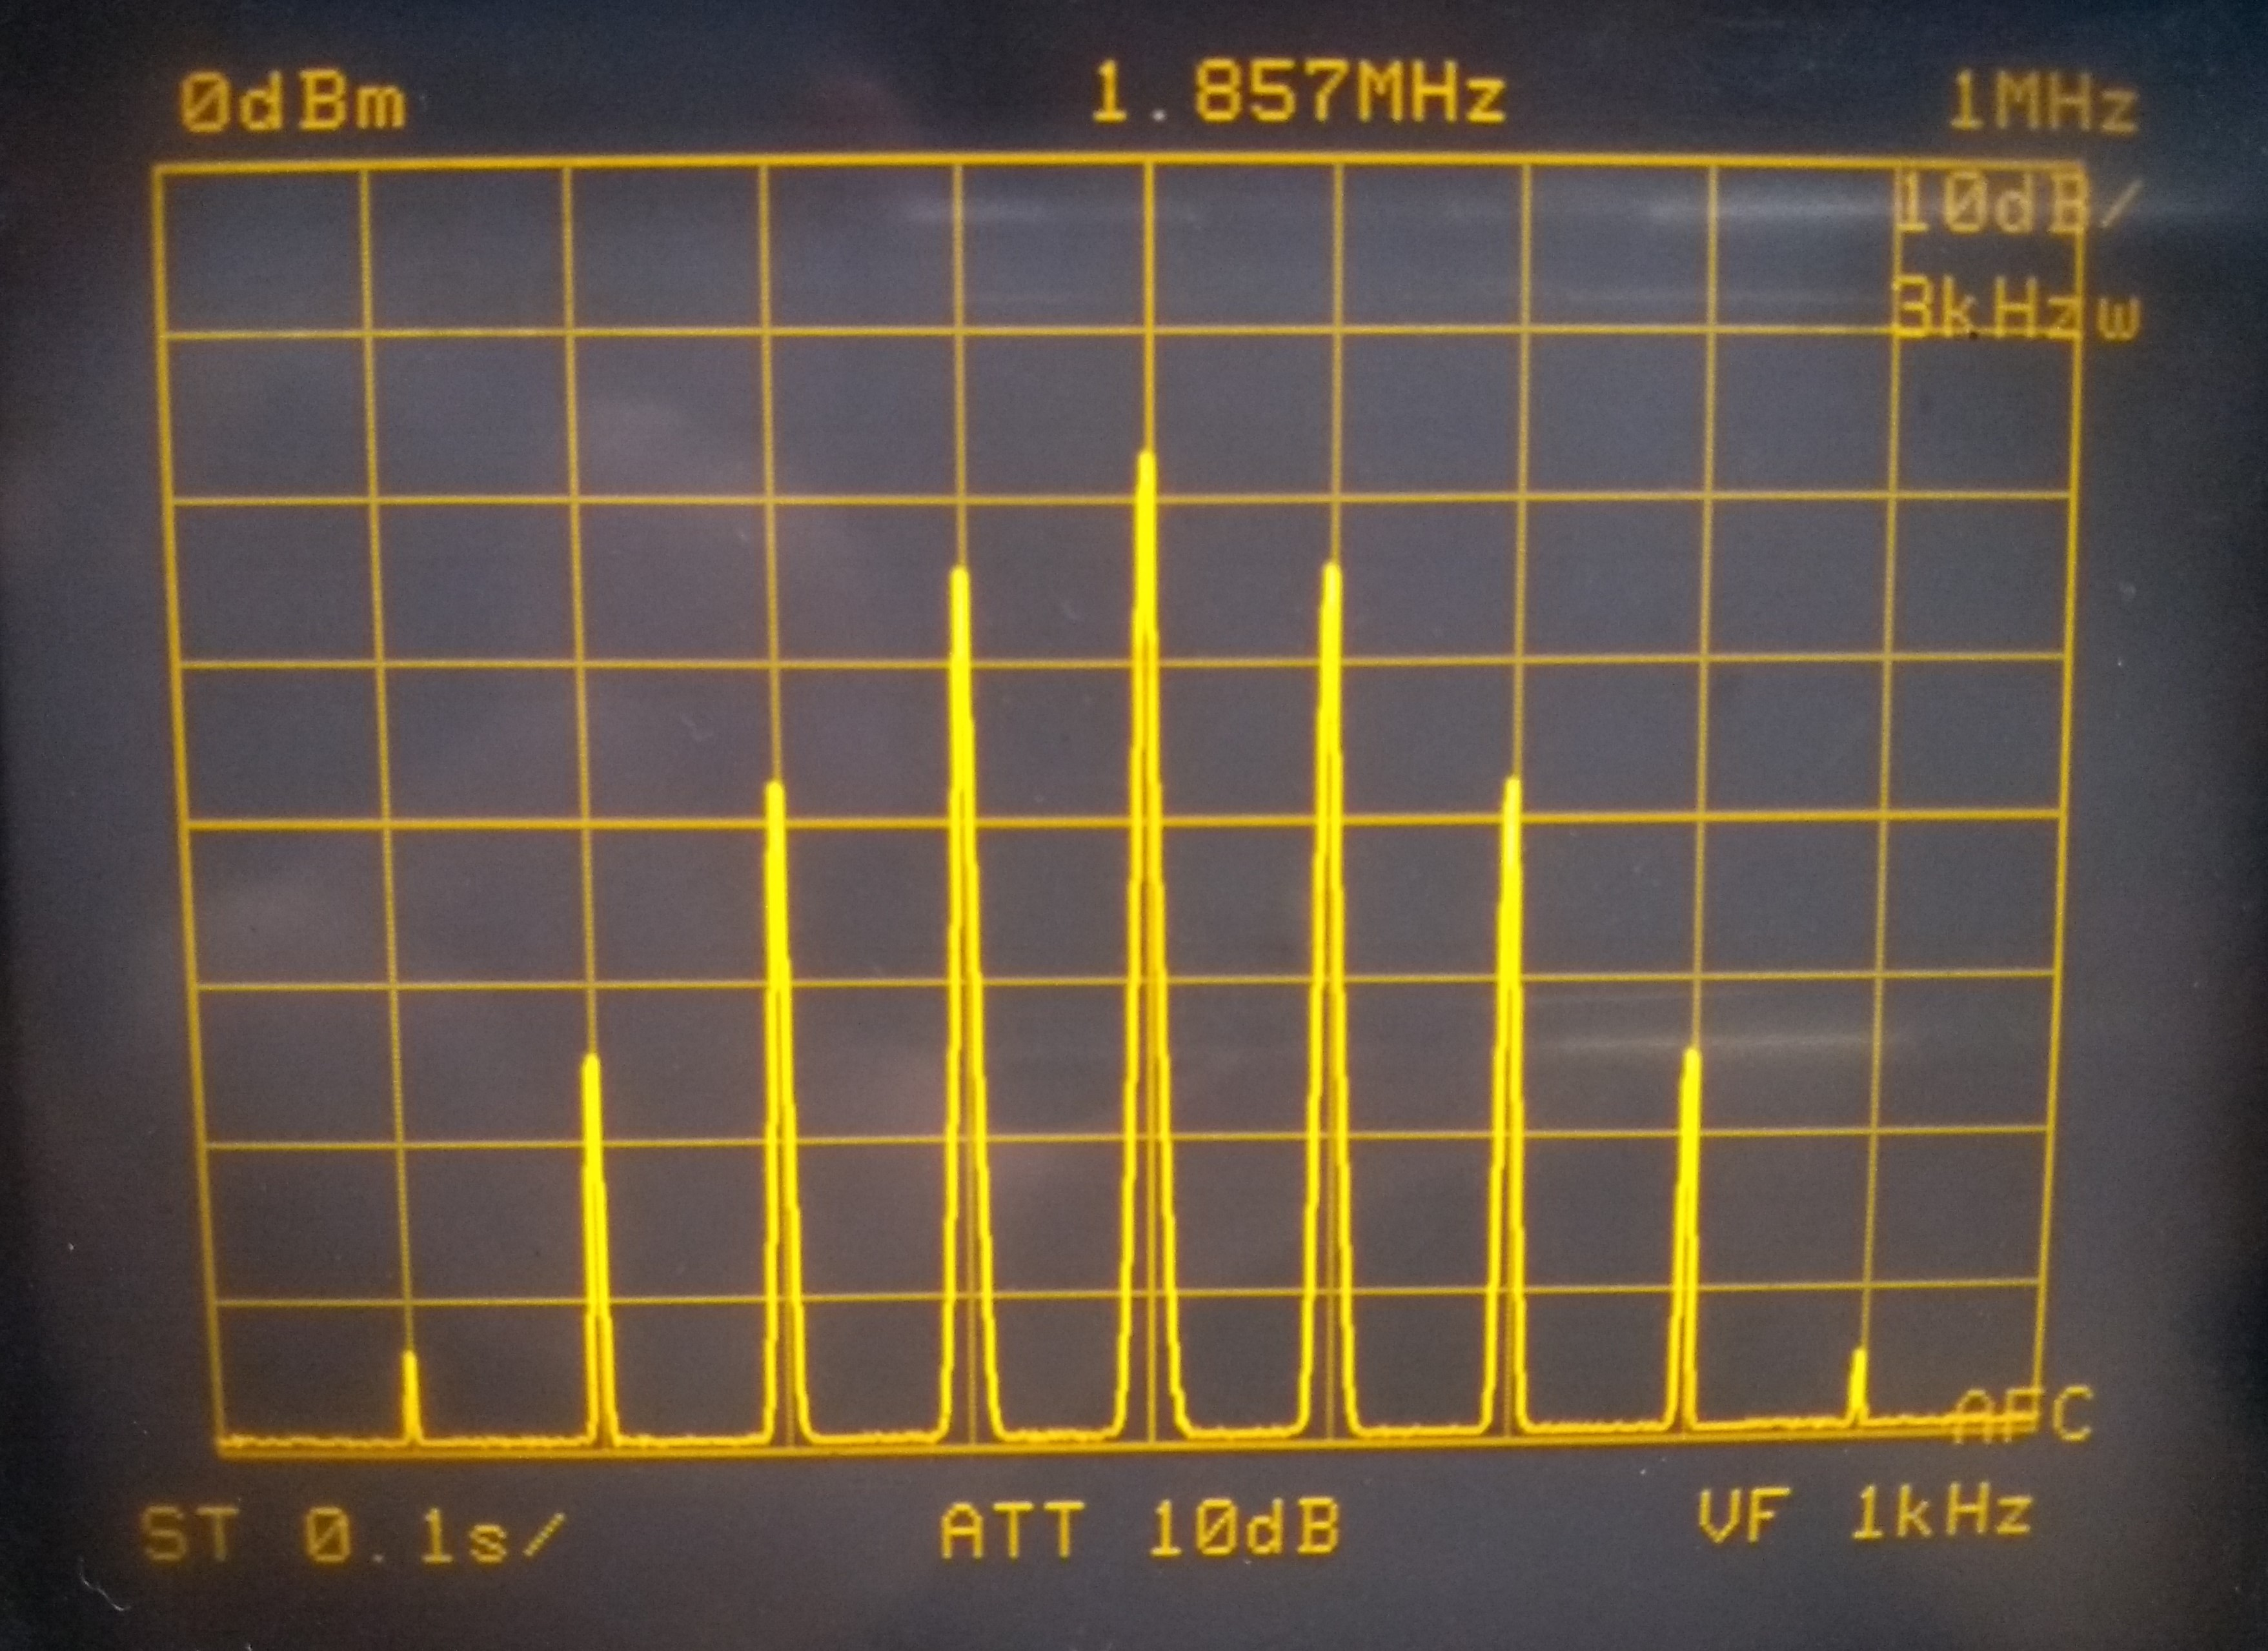
\includegraphics[scale=0.063]{imagenes/labo_tp5_ej4_a_1.jpg}}
	\fbox{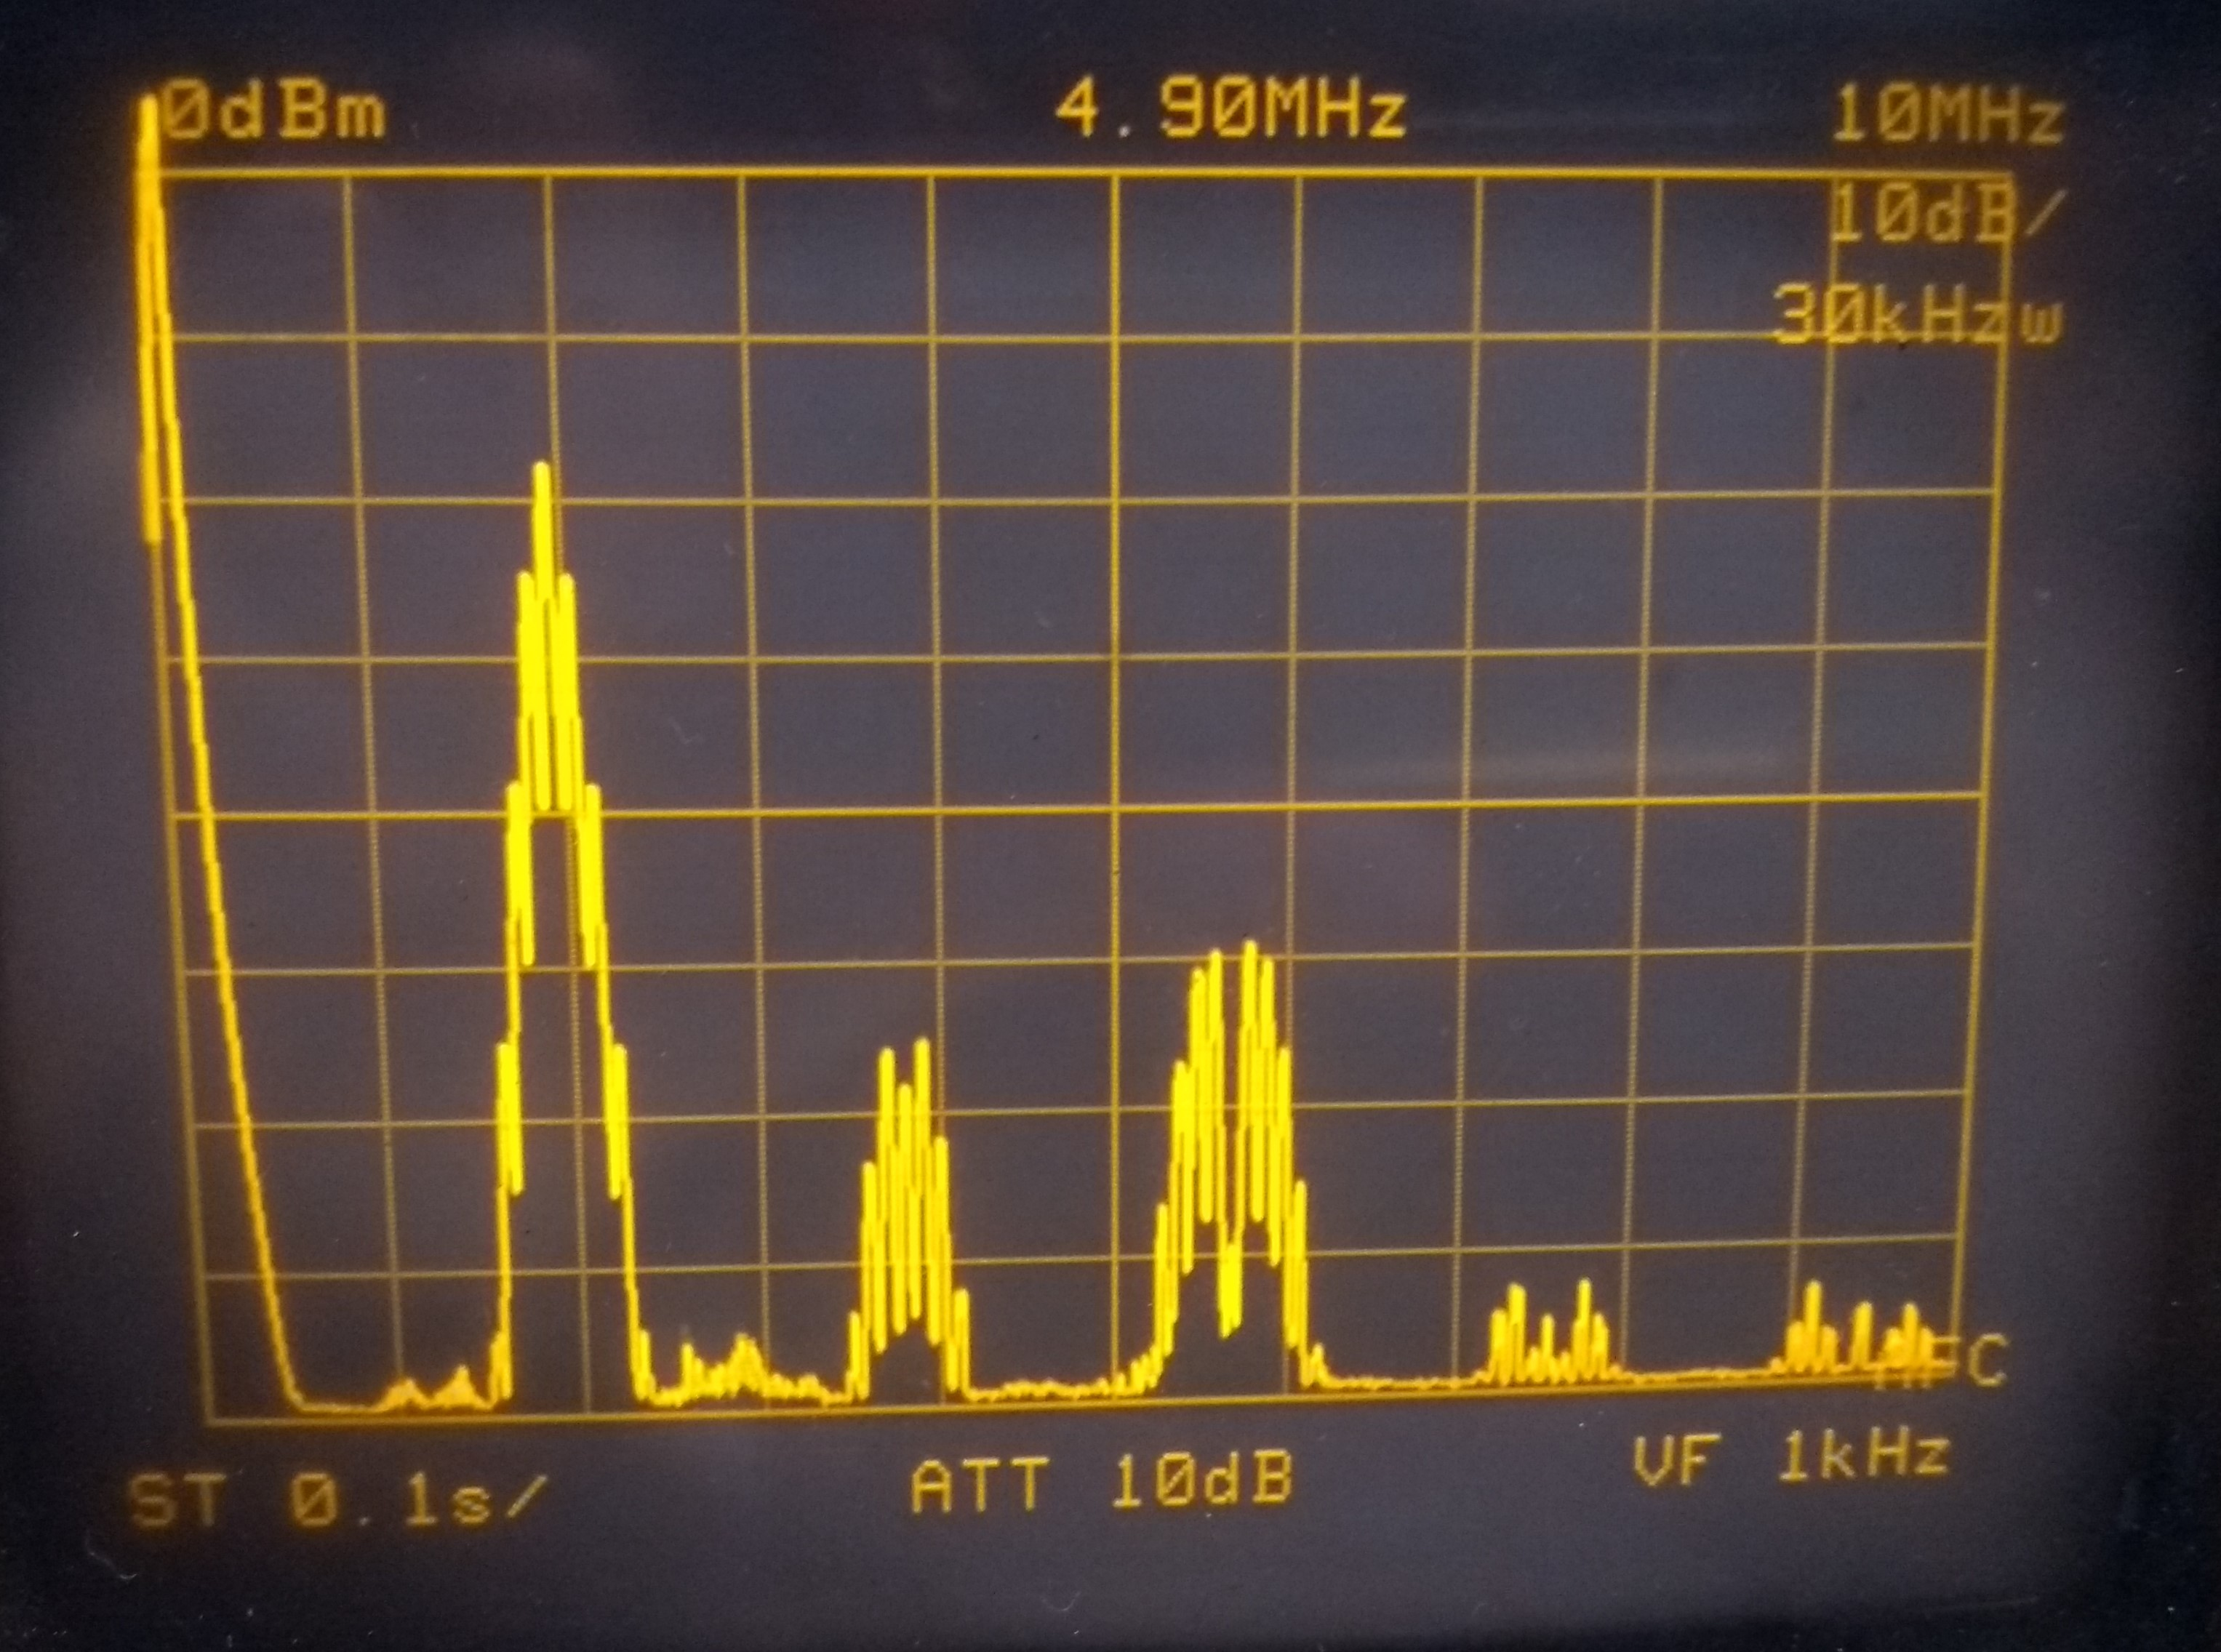
\includegraphics[scale=0.072]{imagenes/labo_tp5_ej4_a_2.jpg}}
	\caption{Espectro de FM con moduladora senoidal}
\end{figure}


Se observaron los cambios al modificar el factor de modulaci\'on de la se\~nal.

\begin{figure}[H]
	\centering
	\fbox{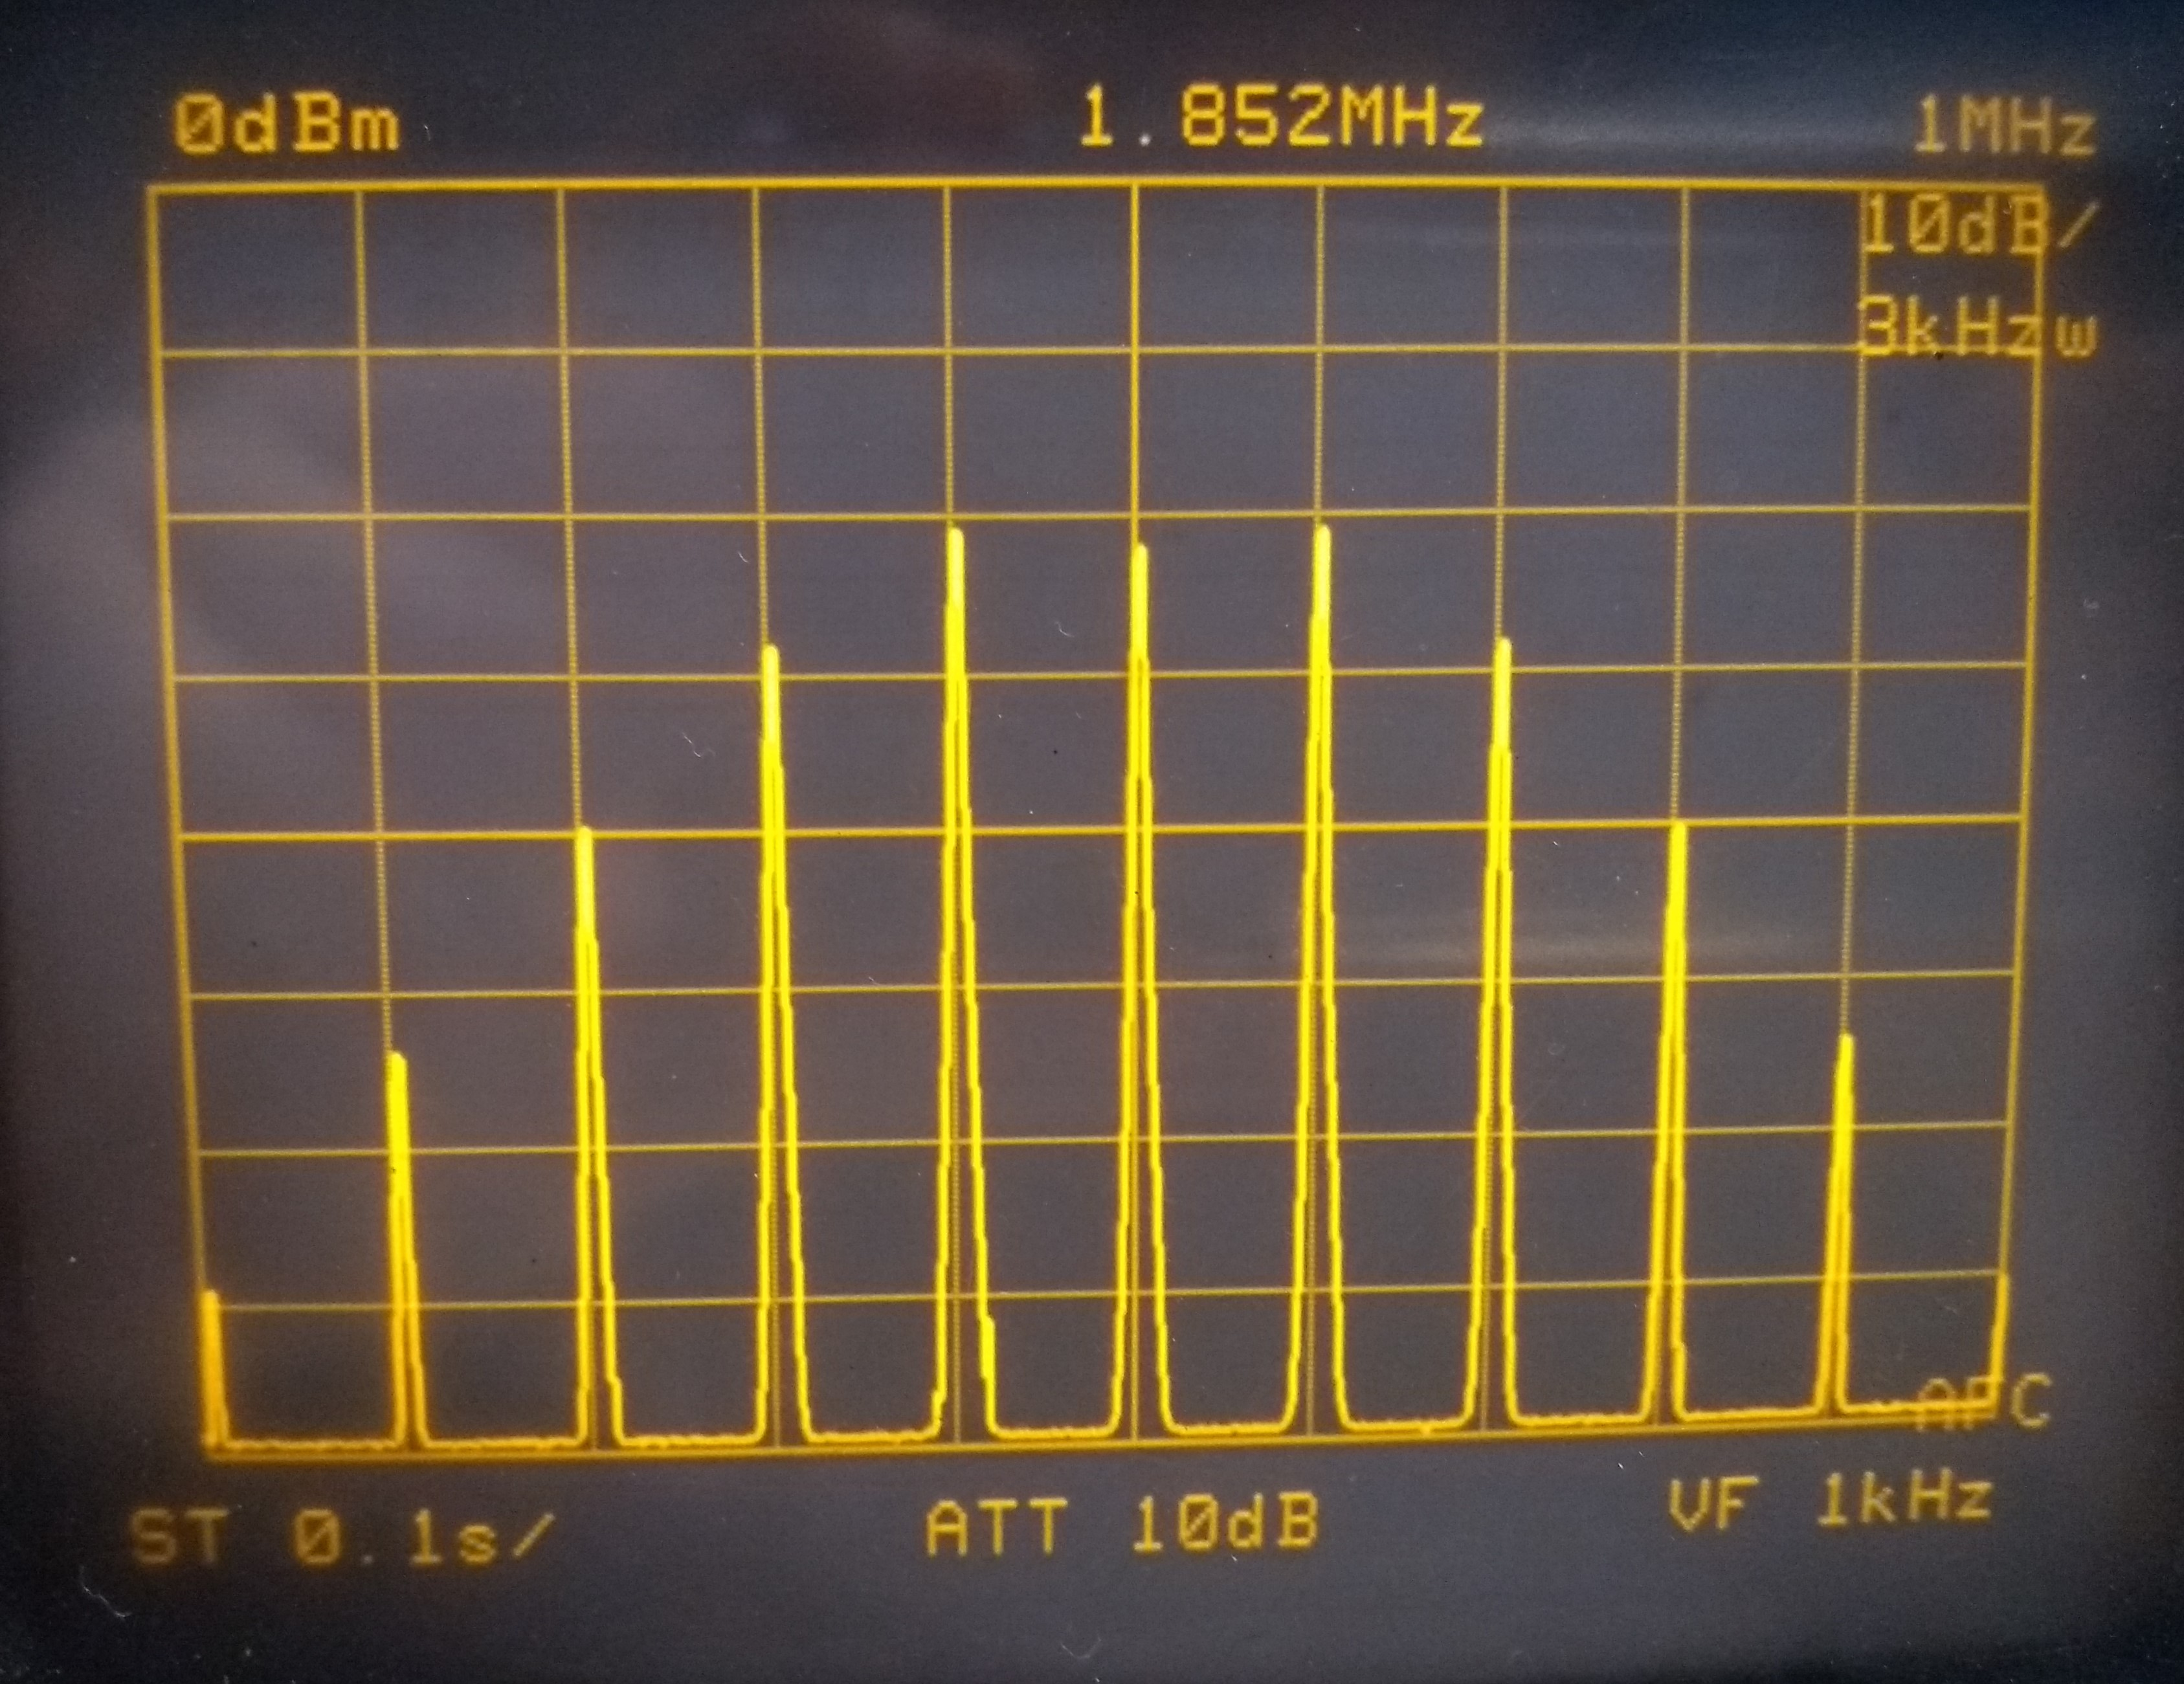
\includegraphics[scale=0.06]{imagenes/labo_tp5_ej4_b_1.jpg}}
	\fbox{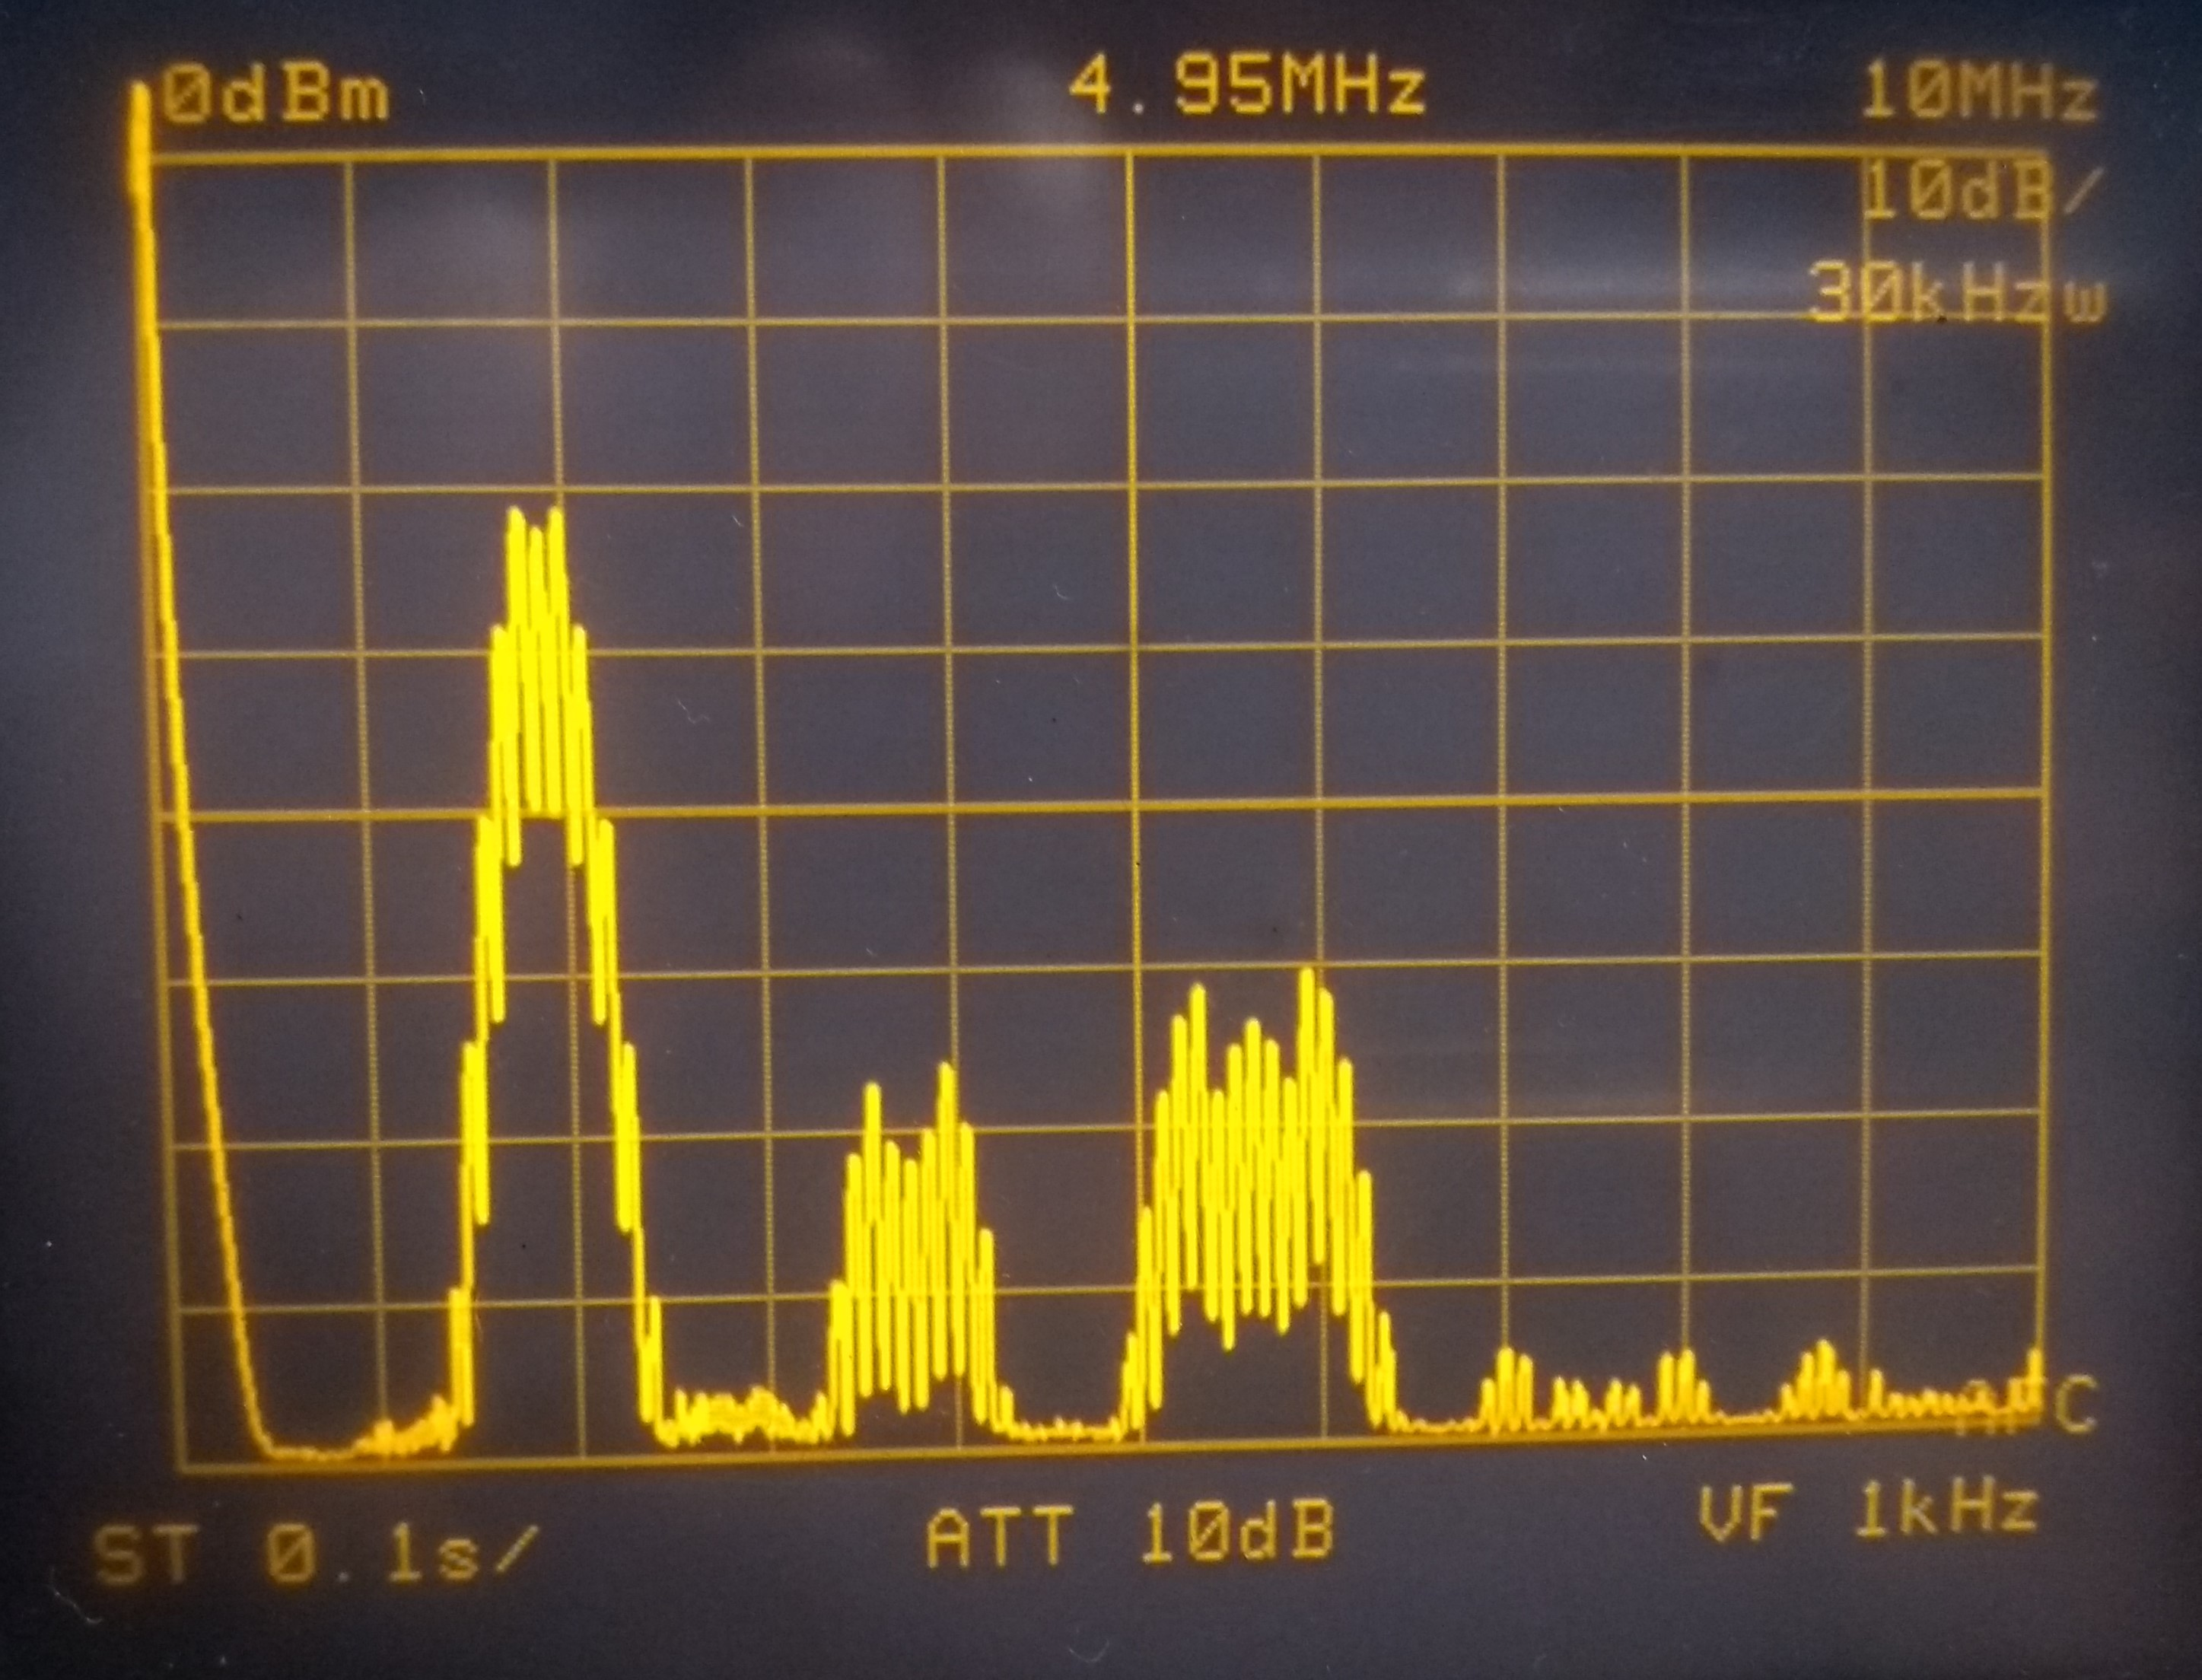
\includegraphics[scale=0.07]{imagenes/labo_tp5_ej4_b_2.jpg}}
	\caption{Espectro de FM con moduladora senoidal}
\end{figure}

En ambos casos, la forma del espectro es la misma, con picos en m\'ultiplos de la frecuencia portadora. Cambia considerablemente, sin embargo, la relaci\'on entre la amplitud de los mismos.\par

Luego se procedi\'o a modular con una se\~nal triangular, tambi\'en de 100kHz.

\begin{figure}[H]
	\centering
	\fbox{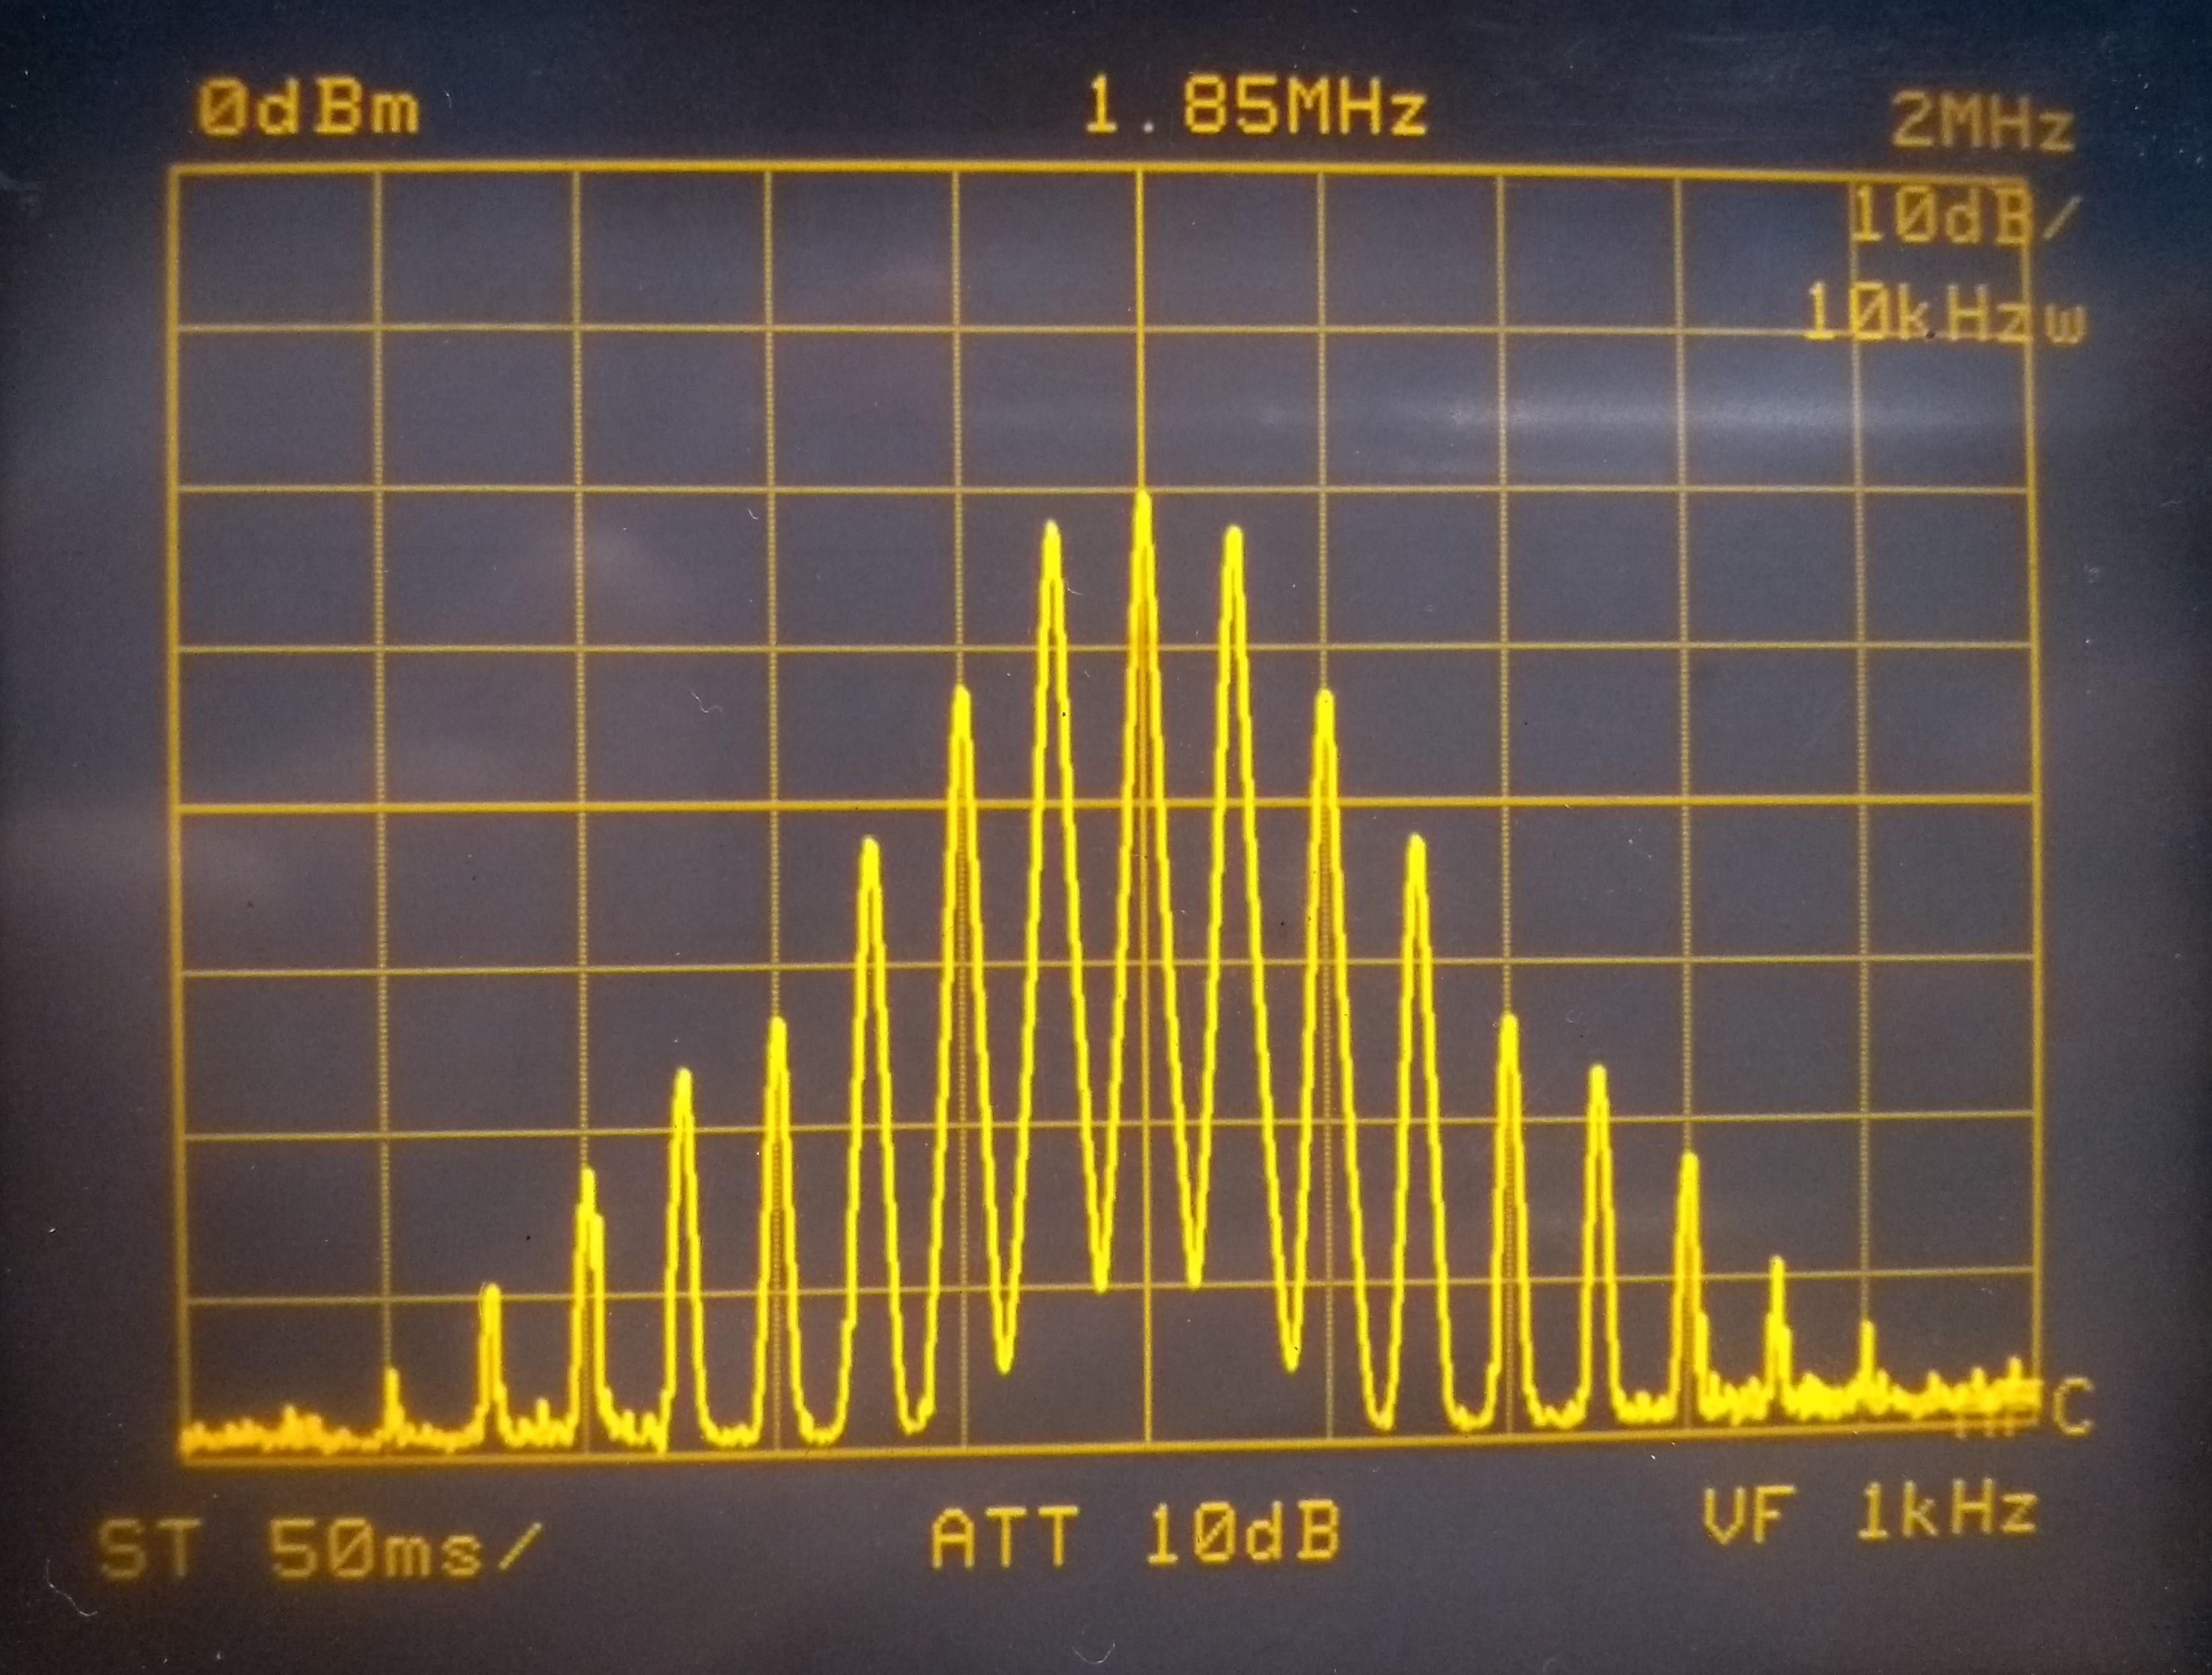
\includegraphics[scale=0.07]{imagenes/labo_tp5_ej4_c_1.jpg}}
	\caption{Espectro de FM con moduladora triangular}
\end{figure}


Por \'ultimo, se observ\'o el espectro cuando tanto la portadora como la moduladora ten\'ian frecuencia de 1.9MHz.
\begin{figure}[H]
	\centering
	\fbox{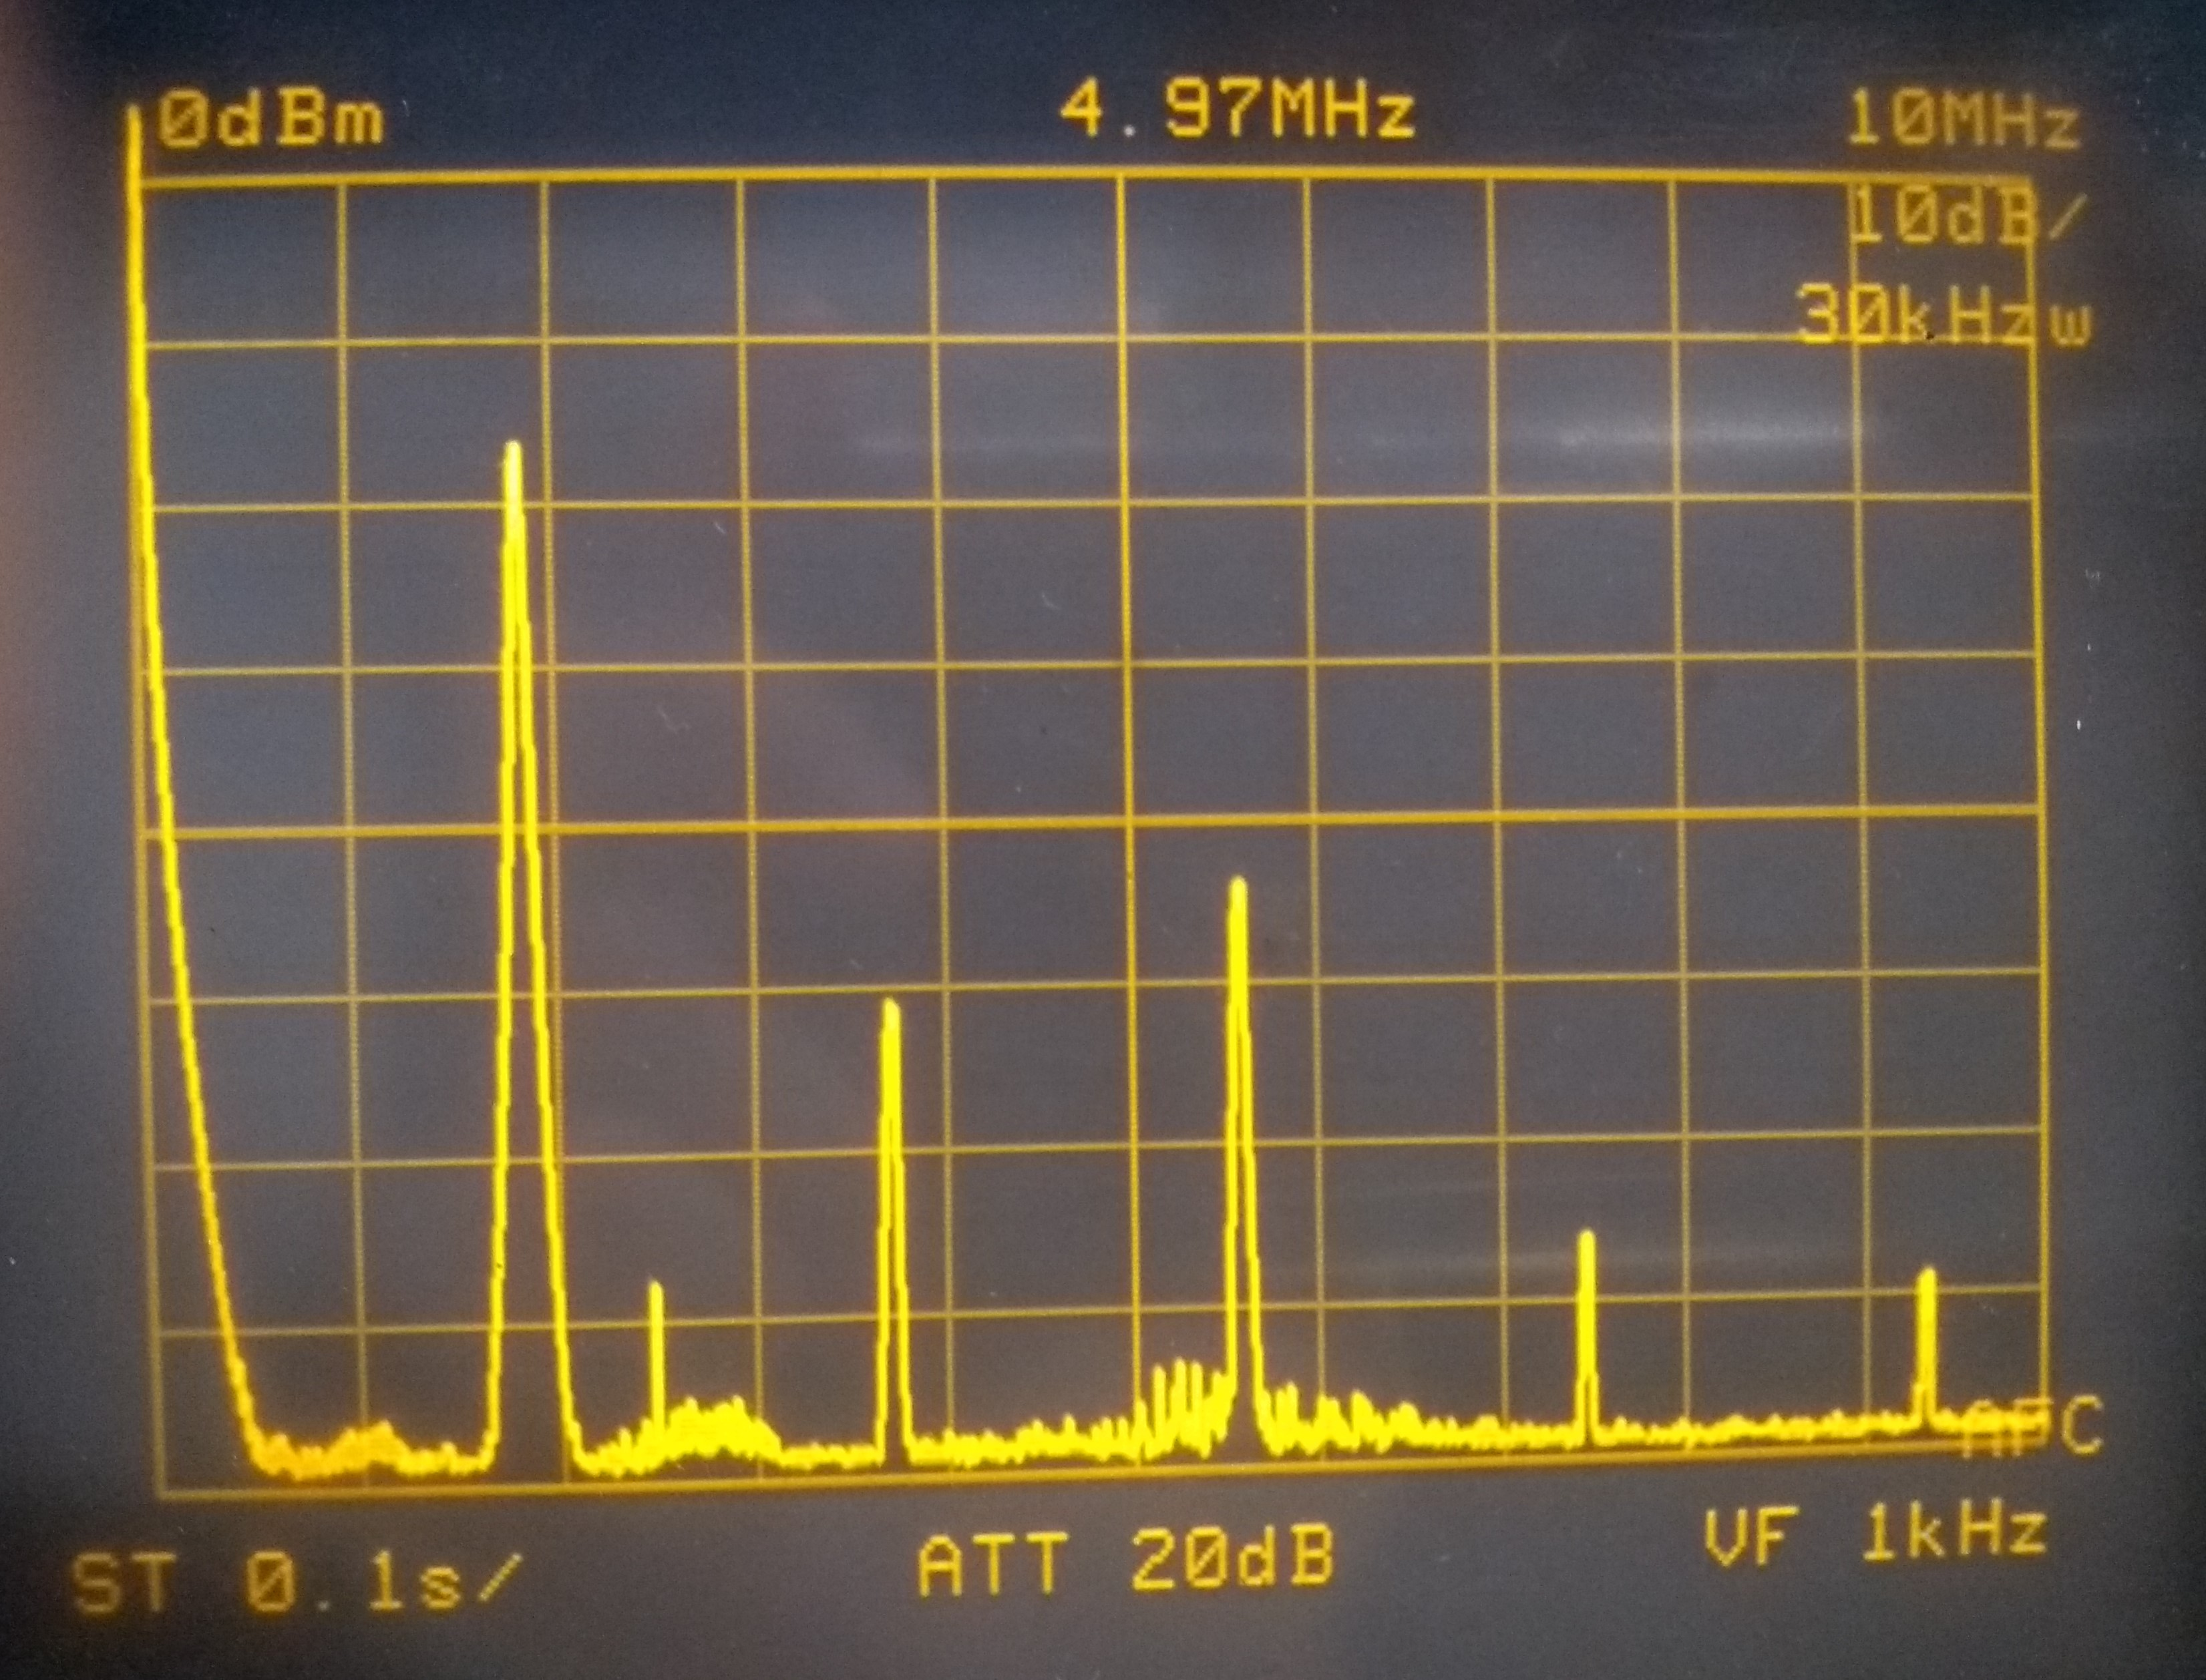
\includegraphics[scale=0.07]{imagenes/labo_tp5_ej4_d.jpg}}
	\caption{Espectro de FM con moduladora senoidal de igual frecuencia que la portadora}
\end{figure}

Cabe destacar que el espectro observado es similar al obtenido para se\~nales moduladas en amplitud en todos los casos.

\end{document}
